 %% Copyright (C) 2011, Andrea Cimino, All Rights Reserved.
 %% This file is distributed under the terms of the Creative Commons
 %% Licence Non-Commercial Share-Alike license


%% Useful stuff for separate compilation.
\ifx\ismaindoc\undefined
\providecommand{\inbpdocument}{
 \documentclass[11pt,a4paper,twoside,titlepage]{scrbook}
%%%%%%%%%%%%%%%%%%%%%%%%%%%%%%%%
%%%%%%%%%%% PACKAGES %%%%%%%%%%%
%%%%%%%%%%%%%%%%%%%%%%%%%%%%%%%%
% encoding
\usepackage[utf8x]{inputenc}
\usepackage[italian]{babel} % babel (suddivisione parole in sillabe)

\usepackage{amsfonts} % matematica
\usepackage{amsmath} % matematica
\usepackage{amssymb} % simboli vari
\usepackage{calrsfs}
\usepackage{caption}
\usepackage{enumerate}
\usepackage{extarrows} % matematica
\usepackage{keyval}
\usepackage{manfnt} % Simboli curva
\usepackage{mathtools} % matematica
\usepackage{multirow} 
\usepackage[usenames, dvipsnames]{color} % colori con nome
\usepackage[pdftex]{graphicx}
\usepackage{epstopdf} % gestione file EPS
\usepackage{wrapfig} % per figure circondate da testo
\usepackage{framed}	% teoremi framed
\usepackage{fancyhdr} % header buffi
\usepackage[T1]{fontenc} % gestione hbox e vbox
\usepackage[a4paper]{geometry}
\usepackage{microtype} % gestione hbox e vbox
\usepackage[thref, amsthm, amsmath, framed, hyperref]{ntheorem} % teoremi (avanzata)
%% \usepackage{prooftree} % gestione prof-tree
\usepackage{rotating}
\usepackage{stmaryrd}
\usepackage{subfig}
\usepackage{syntax} % syntattic stuff
\usepackage{txfonts}
\usepackage{verbatim} % migliorie al verbatim
%\usepackage{hyperref}
%% \usepackage{qtree}
\usepackage{fancyvrb}
\usepackage{listings}
\usepackage{cancel}
\usepackage{tikz}

\usepackage{bbding} %% Icons

%%%%%%%%%%%%%%%%%%%%%%%%%%%%%%%%
%%%%%%%%%%% GEOMETRY %%%%%%%%%%%
%%%%%%%%%%%%%%%%%%%%%%%%%%%%%%%%
\geometry{verbose,tmargin=2cm,bmargin=2.5cm,lmargin=2.5cm,rmargin=2cm}
\parindent0ex %% Remove paragraph indenting

%%%%%%%%%%%%%%%%%%%%%%%%%%%%%%%%
%%%%%%%%%%% CODE ENV %%%%%%%%%%%
%%%%%%%%%%%%%%%%%%%%%%%%%%%%%%%%
% codice
\newcounter{count}
\setcounter{count}{0}
\newenvironment{code}[1]
{
\color{lightgray}\hrulefill\color{code}
\stepcounter{count} {\bf\small Listato di codice \arabic{count}: {#1} }
\verbatim
}
{
\endverbatim
\color{lightgray}\hrulefill
\color{black}
\\
}

% codice semplice
\newenvironment{simplecode}
{
\color{code} \tt
}
{
\rm
}

 % Notation issues

%% Proof trees.
%\input prooftree
\newcommand*{\nohyp}{\phantom{x}}

%% C++.
\newcommand*{\Cplusplus}{{C\nolinebreak[4]\hspace{-.05em}\raisebox{.4ex}
{\tiny\bf ++}}}

%% BNF rules.
\newcommand*{\vbar}{\mathrel{\mid}}

%% Abstract syntax of the analyzed language.
\newcommand*{\Type}{\mathrm{Type}}
\newcommand*{\dType}{\mathrm{dType}}
\newcommand*{\dT}{\mathrm{dT}}
\newcommand*{\sType}{\mathrm{sType}}
\newcommand*{\sT}{\mathrm{sT}}
\newcommand*{\cType}{\mathrm{cType}}
\newcommand*{\cT}{\mathrm{cT}}
\newcommand*{\Integer}{\mathrm{Integer}}
\newcommand*{\Bool}{\mathrm{Bool}}
\newcommand*{\Id}{\mathrm{Id}}
\newcommand*{\id}{\mathrm{id}}
\newcommand*{\rId}{\mathrm{rId}}
\newcommand*{\idx}{\mathrm{x}}
\newcommand*{\ridx}{\underline{\mathrm{x}}}
\newcommand*{\Exp}{\mathrm{Exp}}
\newcommand*{\Exps}{\mathrm{Exps}}
\newcommand*{\Decl}{\mathrm{Decl}}
\newcommand*{\exceptDecl}{\mathrm{exceptDecl}}
\newcommand*{\Catch}{\mathrm{Catch}}
\newcommand*{\Stmt}{\mathrm{Stmt}}
\newcommand*{\Label}{\mathrm{Label}}
\newcommand*{\Con}{\mathrm{Con}}
\newcommand*{\con}{\mathrm{con}}
\newcommand*{\fps}{\mathrm{fps}}
\newcommand*{\funBody}{\mathrm{Body}}
\newcommand*{\funbody}{\mathrm{body}}
\newcommand*{\main}{\mathrm{main}}
\newcommand*{\es}{\mathrm{es}}
\newcommand*{\formParams}{\mathrm{formParams}}
\newcommand*{\emptysequence}{\boxempty}
\newcommand*{\Glob}{\mathrm{Glob}}

%% Sets of configurations
\newcommand*{\NTe}{\Gamma_\mathrm{e}}
\newcommand*{\NTb}{\Gamma_\mathrm{b}}
\newcommand*{\NTd}{\Gamma_\mathrm{d}}
\newcommand*{\NTg}{\Gamma_\mathrm{g}}
\newcommand*{\NTs}{\Gamma_\mathrm{s}}
\newcommand*{\NTk}{\Gamma_\mathrm{k}}
\newcommand*{\Te}{T_\mathrm{e}}
\newcommand*{\Tb}{T_\mathrm{b}}
\newcommand*{\Td}{T_\mathrm{d}}
\newcommand*{\Tg}{T_\mathrm{g}}
\newcommand*{\Ts}{T_\mathrm{s}}
\newcommand*{\Tk}{T_\mathrm{k}}

%% Lambda notation.
\newcommand*{\lambdaop}{\mathop{\lambda}\nolimits}

%% Sets of (no better specified) configurations.
\newcommand*{\NT}[1]{\Gamma_{#1}}
\newcommand*{\NTq}{\Gamma_q}
\newcommand*{\Tq}{T_q}

%% Denotable values.
\newcommand*{\dVal}{\mathrm{dVal}}
%% Storeable values.
\newcommand*{\sVal}{\mathrm{sVal}}
\newcommand*{\sval}{\mathrm{sval}}

%% Control modes.
\newcommand*{\CtrlMode}{\mathord{\mathrm{CtrlMode}}}
\newcommand*{\cm}{\mathrm{cm}}
%% Branch modes.
%\newcommand*{\BranchMode}{\mathord{\mathrm{BranchMode}}}
\newcommand*{\GotoMode}{\mathord{\mathrm{GotoMode}}}
\newcommand*{\SwitchMode}{\mathord{\mathrm{SwitchMode}}}
\newcommand*{\cmgoto}{\mathop{\mathrm{goto}}\nolimits}
\newcommand*{\cmswitch}{\mathop{\mathrm{switch}}\nolimits}
\newcommand*{\cmbreak}{\mathop{\mathrm{break}}\nolimits}
\newcommand*{\cmcontinue}{\mathop{\mathrm{continue}}\nolimits}
\newcommand*{\cmreturn}{\mathop{\mathrm{return}}\nolimits}
%% Exec mode.
\newcommand*{\cmexec}{\mathrm{exec}}
%% Value mode.
\newcommand*{\ValMode}{\mathord{\mathrm{ValMode}}}
\newcommand*{\cmvalue}{\mathop{\mathrm{value}}\nolimits}
%% Environment mode.
\newcommand*{\EnvMode}{\mathord{\mathrm{EnvMode}}}
\newcommand*{\cmenv}{\mathrm{env}}
%% Exception modes.
\newcommand*{\ExceptMode}{\mathord{\mathrm{ExceptMode}}}
\newcommand*{\cmexcept}{\mathrm{except}}

%% Control states.
\newcommand*{\CtrlState}{\mathord{\mathrm{CtrlState}}}
\newcommand*{\cs}{\mathord{\mathrm{cs}}}
%% Value states.
\newcommand*{\ValState}{\mathord{\mathrm{ValState}}}
\newcommand*{\valstate}{\upsilon}
%% Environment states.
%\newcommand*{\EnvState}{\mathord{\mathrm{EnvState}}}
%% Exception states.
\newcommand*{\ExceptState}{\mathord{\mathrm{ExceptState}}}
\newcommand*{\exceptstate}{\varepsilon}

%% Keywords.
\newcommand*{\kw}[1]{\mathop{\textup{\textbf{#1}}}}

\newcommand*{\bop}{\mathbin{\mathrm{bop}}}
%\newcommand*{\uop}{\mathop{\mathrm{uop}}}

%% Things that hold by definition.
\newcommand{\defrel}[1]{\mathrel{\buildrel \mathrm{def} \over {#1}}}
\newcommand{\defeq}{\defrel{=}}
\newcommand{\defiff}{\defrel{\Longleftrightarrow}}
%\newcommand{\defeq}{=}
%\newcommand{\defiff}{\Longleftrightarrow}

%% Divergence relation
\newcommand{\diverges}{\,\mathord{\buildrel \infty \over \longrightarrow}}

%% Special letters denoting sets and algebras.
\providecommand*{\Nset}{\mathbb{N}}             % Naturals
\providecommand*{\Qset}{\mathbb{Q}}             % Rationals
\providecommand*{\Zset}{\mathbb{Z}}             % Integers
\providecommand*{\Rset}{\mathbb{R}}             % Reals

%% Calligraphic alphabet.
\newcommand*{\calA}{\ensuremath{\mathcal{A}}}
\newcommand*{\calB}{\ensuremath{\mathcal{B}}}
\newcommand*{\calC}{\ensuremath{\mathcal{C}}}
\newcommand*{\calD}{\ensuremath{\mathcal{D}}}
\newcommand*{\calE}{\ensuremath{\mathcal{E}}}
\newcommand*{\calF}{\ensuremath{\mathcal{F}}}
\newcommand*{\calG}{\ensuremath{\mathcal{G}}}
\newcommand*{\calH}{\ensuremath{\mathcal{H}}}
\newcommand*{\calI}{\ensuremath{\mathcal{I}}}
\newcommand*{\calJ}{\ensuremath{\mathcal{J}}}
\newcommand*{\calK}{\ensuremath{\mathcal{K}}}
\newcommand*{\calL}{\ensuremath{\mathcal{L}}}
\newcommand*{\calM}{\ensuremath{\mathcal{M}}}
\newcommand*{\calN}{\ensuremath{\mathcal{N}}}
\newcommand*{\calO}{\ensuremath{\mathcal{O}}}
\newcommand*{\calP}{\ensuremath{\mathcal{P}}}
\newcommand*{\calQ}{\ensuremath{\mathcal{Q}}}
\newcommand*{\calR}{\ensuremath{\mathcal{R}}}
\newcommand*{\calS}{\ensuremath{\mathcal{S}}}
\newcommand*{\calT}{\ensuremath{\mathcal{T}}}
\newcommand*{\calU}{\ensuremath{\mathcal{U}}}
\newcommand*{\calV}{\ensuremath{\mathcal{V}}}
\newcommand*{\calW}{\ensuremath{\mathcal{W}}}
\newcommand*{\calX}{\ensuremath{\mathcal{X}}}
\newcommand*{\calY}{\ensuremath{\mathcal{Y}}}
\newcommand*{\calZ}{\ensuremath{\mathcal{Z}}}

%% Declarators for functions and relations.
\newcommand*{\reld}[3]{\mathord{#1}\subseteq#2\times#3}
\newcommand*{\fund}[3]{\mathord{#1}\colon#2\to#3}
\newcommand*{\pard}[3]{\mathord{#1}\colon#2\rightarrowtail#3}

%% Logical quantifiers stuff.
\newcommand{\st}{\mathrel{.}}
\newcommand{\itc}{\mathrel{:}}

%% Domain, codomain and range of a function.
\newcommand*{\dom}{\mathop{\mathrm{dom}}\nolimits}
%\newcommand*{\cod}{\mathop{\mathrm{cod}}\nolimits}
%\newcommand*{\range}{\mathop{\mathrm{range}}\nolimits}

%% Restriction of a function.
\newcommand*{\restrict}[1]{\mathop{\mid}\nolimits_{#1}}

%% Type of a constant.
\newcommand*{\type}{\mathop{\mathrm{type}}\nolimits}

%% Lubs, glbs, and fixed points.
\newcommand*{\lub}{\mathop{\mathrm{lub}}\nolimits}
%\newcommand*{\glb}{\mathop{\mathrm{glb}}\nolimits}
\newcommand*{\lfp}{\mathop{\mathrm{lfp}}\nolimits}
\newcommand*{\gfp}{\mathop{\mathrm{gfp}}\nolimits}

%% Generic widening.
\newcommand*{\widen}{\mathbin{\nabla}}

%% Set theory.
\renewcommand{\emptyset}{\varnothing}

%\newcommand*{\wpc}{\mathop{\wp_\mathrm{c}}\nolimits}
%\newcommand*{\wpf}{\mathop{\wp_\mathrm{f}}\nolimits}
%\newcommand*{\wpn}{\mathop{\wp_\mathrm{n}}\nolimits}

\newcommand*{\sseq}{\subseteq}
\newcommand*{\sseqf}{\mathrel{\subseteq_\mathrm{f}}}
\newcommand*{\sslt}{\subset}
%\newcommand*{\Sseq}{\supseteq}
%\newcommand*{\Ssgt}{\supset}

%\newcommand{\Nsseq}{\nsubseteq}

\newcommand*{\union}{\cup}
\newcommand*{\bigunion}{\bigcup}
%\newcommand*{\biginters}{\bigcap}
\newcommand*{\inters}{\cap}
\newcommand*{\setdiff}{\setminus}

\newcommand{\sset}[2]{{\renewcommand{\arraystretch}{1.2}
                      \left\{\,#1 \,\left|\,
                               \begin{array}{@{}l@{}}#2\end{array}
                      \right.   \,\right\}}}

%% Base sets.
\newcommand*{\ttv}{\mathrm{tt}}
\newcommand*{\ffv}{\mathrm{ff}}
\newcommand*{\divop}{\mathbin{/}}
\newcommand*{\modop}{\mathbin{\%}}
\newcommand*{\andop}{\mathbin{\textbf{\textup{and}}}}
\newcommand*{\orop}{\mathbin{\textbf{\textup{or}}}}
\newcommand*{\notop}{\mathop{\textbf{\textup{not}}}}

\newcommand*{\FI}{\mathop{\mathrm{FI}}\nolimits}
\newcommand*{\DI}{\mathop{\mathrm{DI}}\nolimits}
\newcommand*{\SL}{\mathop{\mathrm{SL}}\nolimits}
%\newcommand*{\match}{\mathop{\mathrm{match}}\nolimits}

\newcommand*{\Env}{\mathord{\mathrm{Env}}}
\newcommand*{\emptystring}{\mathord{\epsilon}}

%% Exceptions.
\newcommand*{\RTSExcept}{\mathord{\mathrm{RTSExcept}}}
\newcommand*{\rtsexcept}{\chi}
\newcommand*{\Except}{\mathord{\mathrm{Except}}}
\newcommand*{\except}{\xi}
\newcommand*{\none}{\mathtt{none}}
\newcommand*{\divbyzero}{\mathtt{divbyzero}}
\newcommand*{\stkovflw}{\mathtt{stkovflw}}
\newcommand*{\datovflw}{\mathtt{datovflw}}
\newcommand*{\memerror}{\mathtt{memerror}}
%\newcommand*{\inerror}{\mathtt{inerror}}
%\newcommand*{\nullptr}{\mathtt{nullptr}}
%\newcommand*{\outofboundsptr}{\mathtt{outofboundsptr}}

%% Flags for terminal configurations of catch clauses.
\newcommand*{\caught}{\mathtt{caught}}
\newcommand*{\uncaught}{\mathtt{uncaught}}

%% Static semantics.
\newcommand*{\TEnv}{\mathord{\mathrm{TEnv}}}
\newcommand*{\tinteger}{\mathrm{integer}}
\newcommand*{\tboolean}{\mathrm{boolean}}
\newcommand*{\trtsexcept}{\mathrm{rts\_exception}}

%% Memory structures.
\newcommand*{\Loc}{\mathord{\mathrm{Loc}}}
\newcommand*{\Ind}{\mathrm{Ind}}
\newcommand*{\Addr}{\mathrm{Addr}}
\newcommand*{\Map}{\mathrm{Map}}
%\newcommand*{\eMap}{\mathrm{eMap}}
\newcommand*{\Stack}{\mathord{\mathrm{Stack}}}
\newcommand*{\Mem}{\mathord{\mathrm{Mem}}}
\newcommand*{\stknew}{\mathop{\mathrm{new}_\mathrm{s}}\nolimits}
\newcommand*{\datnew}{\mathop{\mathrm{new}_\mathrm{d}}\nolimits}
\newcommand*{\txtnew}{\mathop{\mathrm{new}_\mathrm{t}}\nolimits}
\newcommand*{\heapnew}{\mathop{\mathrm{new}_\mathrm{h}}\nolimits}
\newcommand*{\heapdel}{\mathop{\mathrm{delete}_\mathrm{h}}\nolimits}
\newcommand*{\datcleanup}{\mathop{\mathrm{cleanup}_\mathrm{d}}\nolimits}
\newcommand*{\smark}{\mathop{\mathrm{mark}_\mathrm{s}}\nolimits}
\newcommand*{\sunmark}{\mathop{\mathrm{unmark}_\mathrm{s}}\nolimits}
\newcommand*{\slink}{\mathop{\mathrm{link}_\mathrm{s}}\nolimits}
\newcommand*{\sunlink}{\mathop{\mathrm{unlink}_\mathrm{s}}\nolimits}
\newcommand*{\asmark}{\mathop{\mathrm{mark}_\mathrm{s}^\sharp}\nolimits}
\newcommand*{\asunmark}{\mathop{\mathrm{unmark}_\mathrm{s}^\sharp}\nolimits}
\newcommand*{\aslink}{\mathop{\mathrm{link}_\mathrm{s}^\sharp}\nolimits}
\newcommand*{\asunlink}{\mathop{\mathrm{unlink}_\mathrm{s}^\sharp}\nolimits}
\newcommand*{\aswiden}{\mathop{\mathrm{widen}}\nolimits}
\newcommand*{\sm}{\dag}
\newcommand*{\fm}{\ddag}
\newcommand*{\topmost}{\mathop{\mathrm{tf}}\nolimits}
%% Short forms of \datcleanup, \sunmark, \sunlink for table.
\newcommand*{\datcleanupshort}{\mathop{\mathrm{cu}_\mathrm{d}}\nolimits}
\newcommand*{\sunmarkshort}{\mathop{\mathrm{um}_\mathrm{s}}\nolimits}
\newcommand*{\sunlinkshort}{\mathop{\mathrm{ul}_\mathrm{s}}\nolimits}

\newcommand*{\location}[1]{\mathord{#1 \; \mathrm{loc}}}
%\newcommand*{\saeval}{\mathop{\mathrm{aeval}}\nolimits}
%\newcommand*{\saupd}{\mathop{\mathrm{aupd}}\nolimits}
\newcommand*{\asupported}{\mathop{\mathrm{supported}^\sharp}\nolimits}
\newcommand*{\aeval}{\mathop{\mathrm{eval}^\sharp}\nolimits}
\newcommand*{\ceval}[1]{\mathop{\mathrm{eval}_{#1}}\nolimits}

%% Abstracts.
\newcommand*{\Abstract}{\mathord{\mathrm{Abstract}}}
\newcommand*{\abs}{\mathord{\mathrm{abs}}}

%% Integer part function.
\newcommand{\intp}{\mathop{\mathrm{int}}\nolimits}

%% Concrete functions and operations.
% Aritmethic
%% \newcommand*{\conadd}{\mathbin{\boxplus}}
%% \newcommand*{\consub}{\mathbin{\boxminus}}
%% \newcommand*{\conmul}{\mathbin{\boxdot}}
%% \newcommand*{\condiv}{\mathbin{\boxslash}}
%% \newcommand*{\conmod}{\mathbin{\boxbar}}
% Boolean
%% \newcommand*{\coneq}{\mathbin{\triangleq}}
%% \newcommand*{\conineq}{\mathbin{\trianglelefteq}}
%% \newcommand*{\conneg}{\mathbin{\daleth}}
%% \newcommand*{\conor}{\mathbin{\triangledown}}
%% \newcommand*{\conand}{\mathbin{\vartriangle}}
\newcommand*{\bneg}{\mathop{\neg}\nolimits}

%% Abstract functions and operations.
% Aritmethic
\newcommand*{\absuminus}{\mathop{\ominus}\nolimits}
\newcommand*{\absadd}{\mathbin{\oplus}}
\newcommand*{\abssub}{\mathbin{\ominus}}
\newcommand*{\absmul}{\mathbin{\odot}}
\newcommand*{\absdiv}{\mathbin{\oslash}}
\newcommand*{\absmod}{\mathbin{\obar}}
% Boolean
\newcommand*{\abseq}{\mathrel{\triangleq}}
\newcommand*{\absneq}{\mathrel{\not\triangleq}}
\newcommand*{\absleq}{\mathrel{\trianglelefteq}}
\newcommand*{\abslt}{\mathrel{\vartriangleleft}}
\newcommand*{\absgeq}{\mathrel{\trianglerighteq}}
\newcommand*{\absgt}{\mathrel{\vartriangleright}}
\newcommand*{\absneg}{\mathrel{\circleddash}}
\newcommand*{\absor}{\mathrel{\ovee}}
\newcommand*{\absand}{\mathrel{\owedge}}

%% Summaries for theorem-like environments
\newcommand{\summary}[1]{\textrm{\textbf{\textup{#1}}}}

%% Filter function extracting the relevant and irrelevant parts.
\newcommand*{\sel}{\mathop{\mathrm{sel}}\nolimits}
\newcommand*{\mem}{\mathop{\mathrm{mem}}\nolimits}

%% Modeling definite exceptions.
%\newcommand*{\None}{\mathrm{None}}

%% Strict Cartesian products.
\newcommand*{\stimes}{\otimes}
\newcommand*{\spair}[2]{{#1} \otimes {#2}}
%\newcommand*{\rstimes}{\rtimes}
%\newcommand*{\rspair}[2]{{#1} \rtimes {#2}}
%\newcommand*{\lstimes}{\ltimes}
%\newcommand*{\lspair}[2]{{#1} \ltimes {#2}}

%% Additional syntax for the numeric type extension supplement
\newcommand*{\iT}{\mathrm{iT}}
\newcommand*{\iType}{\mathrm{iType}}
\newcommand*{\tschar}{\mathrm{signed\_char}}
\newcommand*{\tuchar}{\mathrm{unsigned\_char}}
\newcommand*{\flcon}{\mathrm{fl}}
\newcommand*{\Float}{\mathrm{Float}}
\newcommand*{\sccon}{\mathrm{sc}}
\newcommand*{\sChar}{\mathrm{sChar}}
\newcommand*{\uccon}{\mathrm{uc}}
\newcommand*{\uChar}{\mathrm{uChar}}

%% Additional macros for the extension for extra numeric types
%% Floating point types.
\newcommand*{\tfloat}{\mathrm{float}}
%% Numeric types
\newcommand*{\nType}{\mathrm{nType}}
\newcommand*{\nT}{\mathrm{nT}}

%% Additional macros for the extension to pointer and arrays:
%% Elementary types.
\newcommand*{\eType}{\mathrm{eType}}
\newcommand*{\eT}{\mathrm{eT}}
%% Elementary values.
%\newcommand*{\eValue}{\mathrm{eVal}}
%% Array types.
\newcommand*{\aType}{\mathrm{aType}}
\newcommand*{\aT}{\mathrm{aT}}
%% Record types.
\newcommand*{\rType}{\mathrm{rType}}
\newcommand*{\rT}{\mathrm{rT}}
%% Object types.
\newcommand*{\oType}{\mathrm{oType}}
\newcommand*{\oT}{\mathrm{oT}}
%% Function types.
\newcommand*{\fType}{\mathrm{fType}}
\newcommand*{\fT}{\mathrm{fT}}
%% Memory types.
\newcommand*{\mType}{\mathrm{mType}}
\newcommand*{\mT}{\mathrm{mT}}
%% Pointer types.
\newcommand*{\pType}{\mathrm{pType}}
\newcommand*{\pT}{\mathrm{pT}}
%% Offsets.
\newcommand*{\Offset}{\mathrm{Offset}}
\newcommand*{\nooffset}{\boxempty}
\newcommand*{\indexoffset}[1]{\mathopen{\boldsymbol{[}}{#1}\mathclose{\boldsymbol{]}}}
\newcommand*{\fieldoffset}[1]{\mathop{\boldsymbol{.}}{#1}}
%% Lvalues.
\newcommand*{\lValue}{\mathrm{LValue}}
\newcommand*{\lvalue}{\mathrm{lval}}
%% Rvalues.
\newcommand*{\rValue}{\mathrm{RValue}}
\newcommand*{\rvalue}{\mathrm{rval}}
%%
\newcommand*{\pointer}[1]{{#1}\boldsymbol{\ast}}
\newcommand*{\maddress}[1]{\mathop{\&}{#1}}
\newcommand*{\indirection}[1]{\mathop{\boldsymbol{\ast}}{#1}}
%%
\newcommand*{\locnull}{\mathord{l_\mathrm{null}}}
\newcommand*{\ptrmove}{{\mathop{\mathrm{ptrmove}}\nolimits}}
\newcommand*{\ptrdiff}{{\mathop{\mathrm{ptrdiff}}\nolimits}}
\newcommand*{\ptrcmp}{{\mathop{\mathrm{ptrcmp}}\nolimits}}
%%
\newcommand*{\arraysyntax}[3]{\kw{#1} {#2} \kw{of}\,{#3}}
\newcommand*{\arraytype}[2]{\arraysyntax{array}{#1}{#2}}
\newcommand*{\firstof}{{\mathop{\mathrm{firstof}}\nolimits}}
\newcommand*{\arrayindex}{\mathop{\mathrm{index}}\nolimits}
\newcommand*{\locindex}{\mathop{\mathrm{locindex}}\nolimits}
%%
\newcommand*{\recordsyntax}[3]{\kw{#1} {#2} \kw{of}\,{#3}}
\newcommand*{\recordtype}[2]{\recordsyntax{record}{#1}{#2}}
\newcommand*{\field}{\mathop{\mathrm{field}}\nolimits}
\newcommand*{\locfield}{\mathop{\mathrm{locfield}}\nolimits}
%%
\newcommand*{\NTo}{\Gamma_\mathrm{o}}
\newcommand*{\To}{T_\mathrm{o}}
\newcommand*{\NTl}{\Gamma_\mathrm{l}}
\newcommand*{\Tl}{T_\mathrm{l}}
%\newcommand*{\NTr}{\Gamma_\mathrm{r}}
%\newcommand*{\Tr}{T_\mathrm{r}}
%%
\newcommand*{\arraydatnew}{\mathop{\mathrm{newarray}_\mathrm{d}}\nolimits}
\newcommand*{\arraystknew}{\mathop{\mathrm{newarray}_\mathrm{s}}\nolimits}
\newcommand\Cut{\using\sf cut\thickness.08em\justifies}
\newcommand{\maybeeq}{\mathrel{\buildrel \mathrm{?} \over =}}



\makeatletter
\g@addto@macro\@verbatim\footnotesize
\makeatother



%%%%%%%%%%%%%%%%%%%%%%%%%%%%%%%%
%%%%%%%% THEOREMS FORMAT %%%%%%%
%%%%%%%%%%%%%%%%%%%%%%%%%%%%%%%%
% shaded theorems and proofs command
\definecolor{lightgray}{RGB}{230,230,230}
\def\theoremframecommand{\colorbox{lightgray}}

%%% theorems
\theoremstyle{break}
\theoremheaderfont{\normalfont\bfseries}
\theorembodyfont{\itshape}
\theoremsymbol{\ensuremath{\diamondsuit}}
\theoremseparator{\newline}
\newtheorem{theo}{
\includegraphics[scale=0.11]{imgs/book.png}Teorema}[chapter]

%%% propositions
\theoremstyle{break}
\theoremheaderfont{\normalfont\bfseries}
\theorembodyfont{\itshape}
\theoremsymbol{\ensuremath{\diamondsuit}}
\theoremseparator{\newline}
\newshadedtheorem{proposition}{Proposizione}[chapter]

%%% exercises
\theoremstyle{break}
\theoremheaderfont{\normalfont\bfseries}
\theorembodyfont{\itshape}
\theoremsymbol{\ensuremath{\diamondsuit}}
\theoremseparator{\newline}
\newshadedtheorem{exercise}{Esercizio}[chapter]

%%% propositions
\theoremstyle{break}
\theoremheaderfont{\normalfont\bfseries}
\theorembodyfont{\itshape}
\theoremsymbol{\ensuremath{\diamondsuit}}
\theoremseparator{\newline}
\newshadedtheorem{property}{\PencilRightDown $\; $ Propriet\`a}[chapter]

%%% lemmas
\theoremstyle{break}
\theoremheaderfont{\normalfont\bfseries}
\theorembodyfont{\itshape}
\theoremsymbol{\ensuremath{\diamondsuit}}
\theoremseparator{\newline}
\newshadedtheorem{lemma}[theo]{Lemma}

%%% definitions
\theoremstyle{break}
\theoremsymbol{\ensuremath{\clubsuit}}
\theoremseparator{\newline}
\newshadedtheorem{defn}[theo]{Definizione}

%%% examples
\theoremstyle{break}
\theorembodyfont{\itshape}
\theoremsymbol{\ensuremath{\ast}}
\theoremseparator{\newline}
\newshadedtheorem{example}[theo]{Esempio}

%%% observations
\theoremstyle{break}
\theorembodyfont{\itshape}
\theoremsymbol{\ensuremath{\ast}}
\theoremseparator{\newline}
\newshadedtheorem{observation}[theo]{

\includegraphics[scale=0.06]{imgs/lens.png}
Osservazione
}

%%% notations
\newtheorem*{notaz}{Notazione}

%%% proofs
\newenvironment{thproof}
{
\vskip 0.03cm
\begin{small}
\textit{Dimostrazione. }
\color{code}
}
{
\color{black}
\end{small}
$ \square $
\vskip 0.2cm
}

%Notes
\newenvironment{notes}{%
  \def\FrameCommand{\colorbox{yellow}}%
  \MakeFramed {\FrameRestore}

\includegraphics[scale=0.02]{imgs/bulb.png}
 \textbf{Nota} \\
 }%
{\endMakeFramed}

%Work in progress
\newenvironment{workinprogress}{%
  \def\FrameCommand{\colorbox{pink}}%
  \MakeFramed {\FrameRestore}
\lhdbend  \textbf{Work in progress} \\
 }%
{\endMakeFramed}

%Openquestion
\newenvironment{openquestion}{%
  \def\FrameCommand{\colorbox{pink}}%
  \MakeFramed {\FrameRestore}
 \textbf{Domanda aperta} \\
 }%
{\endMakeFramed}

%TODO
\newenvironment{todo}{%
  \def\FrameCommand{\colorbox{pink}}%
  \MakeFramed {\FrameRestore}
 \textbf{TODO} \\
 }%
{\endMakeFramed}

%%%%%%%%%%%%%%%%%%%%%%%%%%%%%%%%
%%%%%%%%%%%% HEADER %%%%%%%%%%%%
%%%%%%%%%%%%%%%%%%%%%%%%%%%%%%%%
\pagestyle{fancy}
% i comandi seguenti impediscono la scrittura in maiuscolo
% dei nomi dei capitoli e dei paragrafi nelle intestazioni
\renewcommand{\chaptermark}[1]{\markboth{#1}{}}
\renewcommand{\sectionmark}[1]{\markright{\thesection\ #1}}
\fancyhf{} % rimuove l'attuale contenuto dell'intestazione
% e del pi\`e di pagina
\fancyhead[LE,RO]{\bfseries\thepage}
\fancyhead[LO]{\bfseries\rightmark}
\fancyhead[RE]{\bfseries\leftmark}
\renewcommand{\headrulewidth}{0.5pt}
\renewcommand{\footrulewidth}{0pt}
\addtolength{\headheight}{0.5pt} % riserva spazio per la linea
\fancypagestyle{plain}{%
\fancyhead{} % ignora, nello stile plain, le intestazioni
\renewcommand{\headrulewidth}{0pt} % e la linea
}


%%%%%%%%%%%%%%%%%%%%%%%%%%%%%%%%
%%%%%%%%%%%% COLORS %%%%%%%%%%%%
%%%%%%%%%%%%%%%%%%%%%%%%%%%%%%%%
\definecolor{code}{gray}{0.3}


%%%%%%%%%%%%%%%%%%%%%%%%%%%%%%%%
%%%%%%%%%%%% NUMBERS %%%%%%%%%%%
%%%%%%%%%%%%%%%%%%%%%%%%%%%%%%%%
\setcounter{tocdepth}{3}
\setcounter{secnumdepth}{3}


%%%%%%%%%%%%%%%%%%%%%%%%%%%%%%%%
%%%%%%%%%%% DOC DATA %%%%%%%%%%%
%%%%%%%%%%%%%%%%%%%%%%%%%%%%%%%%
\title{Appunti di MNO}
\author{Gruppo Informatici Rampanti}
\date{ott 2010 - mag 2011}

\pdfinfo{%
  /Title    (Appunti di MNO)
  /Author   (Andrea Cimino e Lorenzo Muti)
  /Creator  (Andrea Cimino)
  /Producer (Lorenzo Muti)
  /Subject  (MNO)
  /Keywords (MNO)
}


%%%%%%%%%%%%%%%%%%%%%%%%%%%%%%%%
%%%%%%%%%%%%% UTILS %%%%%%%%%%%%
%%%%%%%%%%%%%%%%%%%%%%%%%%%%%%%%
% binary symbols
\newcommand{\modder}{\vdash _{R}}

% vertical gaps
\newcommand{\askip}{\vspace{0.5cm}}
\newcommand{\bskip}{\vspace{1.0cm}}

% various symbols
\newcommand{\qedhere}{\ensuremath{\Box}}
\newcommand{\qed}{\hfill \ensuremath{\Box}}

% substitution
\newcommand{\subst}[2]{^{#1} / _{#2}}

% denotational semantics function names
\newcommand{\bbracket}[1]{\left\llbracket #1 \right\rrbracket}

\newcommand{\aexpr}{\mathcal{A}}
\newcommand{\bexpr}{\mathcal{B}}
\newcommand{\cexpr}{\mathcal{C}}
\newcommand{\Aexpr}[1]{\mathcal{A} \bbracket{#1}}
\newcommand{\Bexpr}[1]{\mathcal{B} \bbracket{#1}}
\newcommand{\Cexpr}[1]{\mathcal{C} \bbracket{#1}}

\newcommand{\semdomset}[1]{(V_{#1})_{\bot}}

% semantic evaluations
\newcommand{\opereval}[3]{\left\langle #1, #2 \right\rangle \rightarrow #3}
\newcommand{\denaeval}[3]{\Aexpr{#1} #2 = #3}
\newcommand{\denbeval}[3]{\Bexpr{#1} #2 = #3}
\newcommand{\denceval}[3]{\Cexpr{#1} #2 = #3}

% rotated sqsubseteqs
\newcommand{\upsqsubseteq}{ $\begin{rotate}{90} $\sqsubseteq$ \end{rotate}$ }
\newcommand{\downsqsubseteq}{ $\begin{rotate}{270} $\sqsubseteq$ \end{rotate}$ }

% Space after paragraph declaration
\makeatletter
\renewcommand\paragraph{\@startsection{paragraph}{4}{\z@}%
  {-3.25ex\@plus -1ex \@minus -.2ex}%
  {1.5ex \@plus .2ex}%
  {\normalfont\normalsize\bfseries}}
\makeatother



% fast theorem and definition
\newcommand{\ftheo}[1]{\colorbox{YellowGreen}{#1}}
\newcommand{\fdefn}[1]{\colorbox{SkyBlue}{#1}}

\theoremstyle{break}
\theoremsymbol{\ensuremath{\clubsuit}}
\theoremseparator{\newline}
\newshadedtheorem{proc}[theo]{Procedura}

% bold math!
\newcommand{\bm}[1]{\mbox{\boldmath{$#1$}}}

\newcommand{\positive}[1]{\textbf{\color{green} +} #1}
\newcommand{\negative}[1]{\textbf{\color{red} -} #1}


\newtheoremlisttype{tab}%
{\begin{tabular*}{\linewidth}{@{}lrl@{\extracolsep{\fill}}r@{}}}%
{##1&##2&##3&##4\\}%
{\end{tabular*}}
\begin{document}
}
\providecommand{\outbpdocument}{\end{document}}
\else
\providecommand{\inbpdocument}{}
\providecommand{\outbpdocument}{}
\fi



\inbpdocument 

\chapter{Metodi di risoluzione per sistemi non lineari}
Andremo adesso a vedere come si possono risolvere i sistemi non
lineari. Per prima cosa caratterizziamoli.

Possiamo definire un sistema non lineare in due maniere: dato $ \Omega
\subseteq \Rset^n $, con $\Omega$ sotto insieme aperto di $\mathbb{R}^{n}$:

\begin{itemize}
\item $ F(\mathbf{x}) = \mathbf{0} \qquad \text{dove } F:\Omega \rightarrow \Rset^n $,
  dove
\[ F(\mathbf{x}) = \left\lbrace \begin{array}{c}
f_1(\mathbf{x}) = 0 \\ f_2(\mathbf{x}) = 0 \\ \vdots \\ f_n(\mathbf{x}) = 0
\end{array}  \right. \]
Le $f_i$ sono quindi funzioni del tipo $\Omega \rightarrow \mathbb{R}$.
\item $ \mathbf{x} = G(\mathbf{x}) \qquad \text{dove } G:\Omega \rightarrow \Rset^n $,
  ovvero
\[ \left\lbrace \begin{array}{c}
x_1 = g_1(\mathbf{x}) \\ 
x_2 = g_2(\mathbf{x}) \\ 
\vdots \\ 
x_n = g_n(\mathbf{x})
\end{array}  \right. \]
Anche le $g_i$ sono quindi funzioni del tipo $\Omega \rightarrow \mathbb{R}$.

\end{itemize}

Inoltre, se $ F(\mathbf{x}),G(\mathbf{x}) \in C^1(\Omega) $, le due funzioni generano le matrici Jacobiane, che chiameremo rispettivamente $ J(\mathbf{x}) $ ed $ H(\mathbf{x})$.

Per arricchire le possibilit\`a di personalizzare il metodo
risolutivo, possiamo porre
 $$ \mathbf{x} = G(\mathbf{x}) = \mathbf{x} - A(\mathbf{x})F(\mathbf{x})$$
per qualche $A(x)$.

Tale relazione si verifica in quanto $F(\mathbf{x}) = \mathbf{0}$ nella soluzione.


\section{Generalit\`a sui metodi iterativi per sistemi non lineari}
Possiamo dunque studiare le propriet\`a generali della famiglia dei
metodi iterativi che seguono lo schema

$$ x^{(i+1)} = G(x^{(i)}) = x^{(i)} - A(x^{(i)})F(x^{(i)}) $$

e che definiscono una successione di $ \mathbf{x}^{(i)} \in \Rset^n $ che
converge ad $ \alpha $ se $ \lim_{i \to \infty} || \mathbf{x}^{(i)}-\alpha
|| = 0 $

Vediamo adesso di capire se e quando questo schema iterativo pu\`o
convergere alla soluzione. Enunciamo un teorema che ci da una
condizione sufficiente per lo schema iterativo $ \mathbf{x}^{(i+1)} =
G(\mathbf{x}^{(i)}) $.

\begin{theo}[Teorema del punto fisso (sufficiente)]
Sia $ \mathbf{x} = G(\mathbf{x}) $ un sistema non lineare, e $ \alpha $ una soluzione di
tale sistema (tale dunque che $ \alpha = G(\mathbf{\alpha}) $). Sia $S$ un
intorno di $ \mathbf{\alpha} $, tale cio\'e che per un certo valore di $ \rho >
0 $ vale
\[ S = \left\lbrace x \in \Rset^n. || \mathbf{x} - \mathbf{\alpha} ||_{\infty} \leq \rho \right\rbrace \]
Sia inoltre
\[ \forall \mathbf{x} \in S.||H(\mathbf{x})||_{\infty} < 1 \]

Allora si ha convergenza per $ \mathbf{x}^{(0)} \in S $.
\end{theo}
\begin{thproof}
Per induzione si dimostra che
$$ || \mathbf{x}^{(i)} - \mathbf{\alpha} ||_{\infty} \leq \lambda^{i}\rho \quad
\text{dove } \lambda = \max_{S}||H(\mathbf{x})||_{\infty} $$

\begin{description}
\item[$ P(0) $] banalmente $ || \mathbf{x}^{(0)} - \alpha ||_{\infty} \leq 1
  \cdot \rho $ \`e  vera per ipotesi
\item[$ P(i) \Rightarrow P(i+1) $] So che $ \mathbf{x}^{(i)} - \mathbf{\alpha} =
  G(\mathbf{x}^{(i-1)}) - G(\alpha) $. Si tratta di un vettore: possiamo
  descrivere la $r$-esima componente, utilizzando il teorema del valor
  medio (\ref{teo-valor-medio-rn}), come
$$ \mathbf{x}^{(i)}_{r} - \alpha_{r} = g_r(\mathbf{x}^{(i-1)}) - g_r(\mathbf{\alpha}) =
 \nabla g_r (\mathbf{\xi}_r) ( \mathbf{x}^{(i-1)} - \mathbf{\alpha} )
 = \displaystyle \sum_{s=1}^{n} \dfrac{\partial g_r}{\partial x_s}(\xi_r)  (x_s^{(i-1)} - \alpha_s)
$$
e
$ \triangledown g_r (\mathbf{\xi}_r) $ \`e la riga $r$-esima della matrice
jacobiana di $G$ calcolata in $ \mathbf{\xi}_r $. Passiamo al modulo:
$$| x_r^{(i)} - \alpha_r | = \left| \displaystyle \sum_{s=1}^{n} \dfrac{\partial g_r}{\partial x_s}(\xi_r)  (x_s^{(i-1)} - \alpha_s) \right| $$
Per la disuguaglianza triangolare tra moduli (\ref{disuguaglianza-triangolare-moduli} a pag. \pageref{disuguaglianza-triangolare-moduli}) si ha:
$$ \left| \displaystyle \sum_{s=1}^{n} \dfrac{\partial g_r}{\partial x_s}(\xi_r)  (x_s^{(i-1)} - \alpha_s) \right| \leq 
\displaystyle \sum_{s=1}^{n} \left|\dfrac{\partial g_r}{\partial x_s}(\xi_r) (x_s^{(i-1)} - \alpha_s) \right| $$
Ricordando che $|ab|=|a|\cdot|b|$, si ha infine
$$| x_r^{(i)} - \alpha_r | \leq \sum^{n}_{s = 1} \left| \dfrac{\partial g_r}{\partial x_s}(\xi_r) \right| \left| x^{(i-1)}_s - \alpha_s \right| $$
Considerando che la norma infinito di un vettore è $|| y ||_{\infty} = \displaystyle \max_{i=1 \cdots n}|y_i|$, si ha
$$\sum^{n}_{s = 1} \left(\left| \dfrac{\partial g_r}{\partial x_s}(\xi_r) \right| \left| x^{(i-1)}_s - \alpha_s \right|\right)
\leq \sum^{n}_{s = 1} \left(\left| \dfrac{\partial g_r}{\partial x_s}(\xi_r) \right| || x^{(i-1)} - \alpha ||_{\infty} \right)
= \sum^{n}_{s = 1} \left(\left| \dfrac{\partial g_r}{\partial x_s}(\xi_r) \right| \right) || x^{(i-1)} - \alpha ||_{\infty}$$

Inoltre, considerando che la norma infinito di una matrice è $|| A ||_{\infty} = \displaystyle \max_{i=1 \cdots n}\sum_{j=1}^n|A_{ij}|$, e quindi $$|| H(x) ||_{\infty}  = \displaystyle \max_{i=1 \cdots n}\displaystyle \sum_{s=1}^{n}\left|\frac{\partial g_i(x)}{\partial x_s}\right|$$ si ha
\[
 \sum^{n}_{s = 1} \left(\left| \dfrac{\partial g_r}{\partial x_s}(\xi_r) \right| \right) || x^{(i-1)} - \alpha ||_{\infty} \leq || H(\xi_r) ||_{\infty}  || \mathbf{x}^{(i-1)} - \mathbf{\alpha} ||_{\infty} \leq \lambda || \mathbf{x}^{(i-1)} - \mathbf{\alpha} ||_{\infty} \]
In definitiva sappiamo che
\[ | x_r^{(i)} - \alpha_r | \leq \lambda || \mathbf{x}^{(i-1)} - 
\mathbf{\alpha} ||_{\infty} \quad r=1 \ldots n \]
questo vale in particolare per $r$ che massimizza  $| x_r^{(i)} - \alpha_r | $
\[ || \mathbf{x}^{(i)} - \mathbf{\alpha} ||_{\infty} \leq \lambda || \mathbf{x}^{(i-1)} - \mathbf{\alpha} ||_{\infty} \]
Possiamo quindi scrivere
\[ || \mathbf{x}^{(i)} - \mathbf{\alpha} ||_{\infty} \leq \lambda || \mathbf{x}^{(i-1)} - \alpha ||_{\infty} \leq \lambda^2 || \mathbf{x}^{(i-2)} - \mathbf{\alpha} ||_{\infty} \leq \ldots \leq \lambda^{(i)} || \mathbf{x}^{(0)} - \mathbf{\alpha} ||_{\infty} \leq \lambda^i \rho \]
in quanto $ \mathbf{x}^{(0)} \in S \Rightarrow ||\mathbf{x}^{(0)} - \mathbf{\alpha} ||_{\infty}
\leq \rho $.
\end{description}

Detto questo, \`e facile vedere che, essendo $ \lambda < 1 $, $
\lambda^i \rho \xrightarrow{i \rightarrow \infty} 0 $ e che quindi $
|| \mathbf{x}^{(i)} - \mathbf{\alpha} ||_{\infty} \xrightarrow{i \rightarrow \infty} 0 $
\end{thproof}

Questo teorema fornisce una condizione sufficiente per la
convergenza. Se quindi si verificano le ipotesi, possiamo affermare
con certezza che il metodo converge. Ma il metodo pu\`o convergere
anche se le condizioni non si verificano!

Vediamo un esempio.

\begin{example}
Consideriamo il sistema non lineare
 $$ \left\{
\begin{array}{l}
 x_1 = g_1(x) = \frac{1}{4}(x_{1}^{2} + x_{2}^{2}) \\ x_2 = g_2(x) =
 \sin(x_1 + 1)
\end{array}
\right. \qquad x= \begin{pmatrix} x_1 \\ x_2
    \end{pmatrix}
$$

Vogliamo

\begin{itemize}
 \item Verificare l'esistenza di punti fissi
 \item Applicare il teorema del punto fisso
\end{itemize}

Tracciamo il grafico delle due funzioni. La prima delle due \`e una
circonferenza, la seconda un seno.

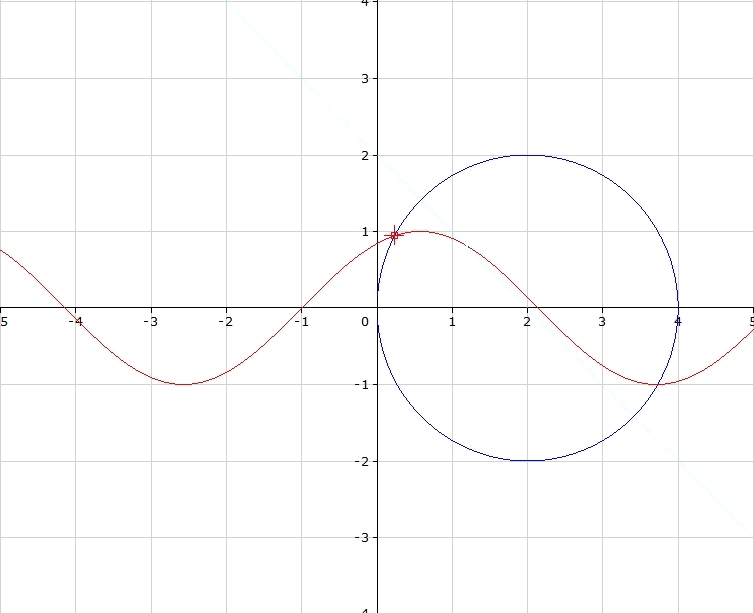
\includegraphics[width=350px]{imgs/121701.jpg}

Come possiamo vedere, ci sono due punti di incontro, che chiameremo $
\alpha $ (quello pi\`u vicino all'asse delle ordinate) e $ \beta
$. Ora devo trovare un intorno S di uno dei due punti tale che $
\forall x \in S.||H(x)||_{\infty} < 1 $. Calcoliamo $ H(x) $, che
ricordiamo essere la matrice la quale, sulle righe, ha i gradienti
delle funzioni che compongono $G$.

$$ H(x) = \left[\begin{array}{cc} \frac{x_1}{2} & \frac{x_2}{2}
    \\ \cos(x_1 +1)& 0
\end{array}          
\right]
$$

Devo ora calcolare la norma infinito della matrice, lasciando $x$
parametrico. La norma infinito \`e la massima somma degli elementi
delle righe di

$$ ||H(x) ||_{\infty} = \max(\frac{1}{2} (|x_{1}| + |x_{2}|), |
cos(x_1 + 1)|) $$

Voglio che $ || H(x) ||_{\infty} $ sia minore di 1: ovviamente $ |
cos(x_1 + 1)| < 1 $, quindi rimane da vedere che $ \frac{1}{2}
(|x_{1}| + |x_{2}|) < 1 $. Questo accade quando $ x_1 + x_2 < 2
$. Possiamo dunque tracciare l'equazione della retta $ y = - x + 2 $
sotto la quale vale sempre $ || H(x) || _{\infty} < 1 $. Possiamo
vedere il grafico di questa retta nella pagina successiva.

Se prendiamo $ \alpha $, appare evidente che possiamo costruirne un
intorno S non vuoto tale che $ \forall x \in S.H(x) < 1 $: basta che
tale intorno non oltrepassi la retta $ x_1 + x_2 < 2 $. Non possiamo
dire la stessa cosa per $ \beta $: infatti $ H(\beta) > 1 $ ed \`e
quindi impossibile costruirne un intorno in cui la propriet\`a non
vada. Ma pu\`o darsi che il metodo funzioni comunque, in quanto la
propriet\`a enunciata \emph{non \`e necessaria}.

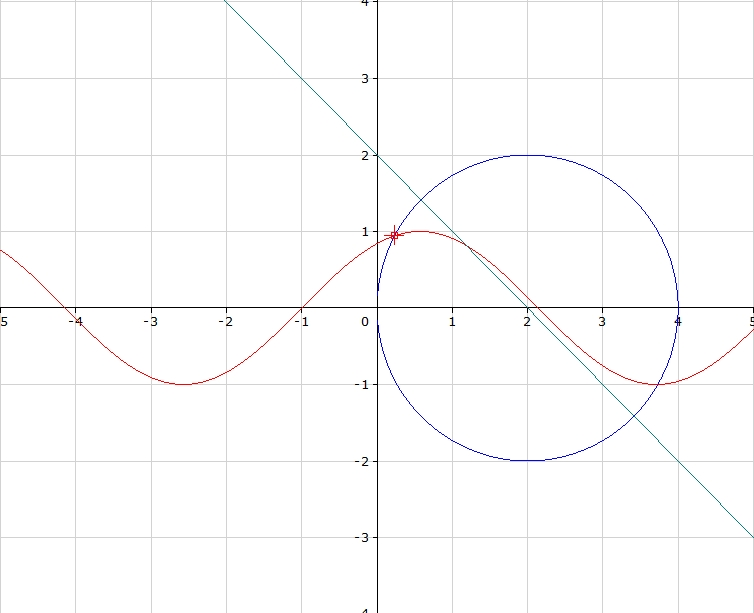
\includegraphics[width=350px]{imgs/121702.jpg}
\end{example}

Enunciamo un secondo teorema del punto fisso, che \`e  necessario e
sufficiente.

\begin{theo}[Teorema del punto fisso (necessario e sufficiente)]\label{theo:ptofisso2}
Siano
\begin{itemize}
\item $g(\mathbf{x})$ di classe $C^{1}(\Omega)$
\item $\Omega$ insieme aperto
\item $ \mathbf{\alpha} $ punto di $ \Omega $ tale che $ \mathbf{\alpha} = g(\mathbf{\alpha}) $
  ($ \mathbf{\alpha} $ \`e punto fisso di $g$)
\end{itemize}
Allora esiste una norma $|| \cdot ||_* $ vettoriale ed un intorno $ S
= \left\lbrace x : || x - \alpha ||_* < \pi \right\rbrace $ tale che
per $\mathbf{x}^{(0)}\in S$ si ha convergenza se e solo se $\rho(H(\mathbf{\alpha}))
\leq 1$.
\end{theo}

Non dimostreremo questo teorema. Piuttosto viene da chiedersi il
perch\'e delle differenze fra i due teoremi: uno pone condizioni sulla
norma, l'altro sul raggio spettrale.

Effettivamente esiste un legame fra queste due grandezze: si veda il Teorema \ref{th:raggio-spettrale-norme-indotte} a pagina \pageref{th:raggio-spettrale-norme-indotte}, il quale asserisce che per ogni matrice $B$ e per ogni norma indotta $|| \cdot ||$ vale
$$ \rho(B) = \inf_{|| \cdot || \text{ indotta}}\{ ||B||\}$$

In particolare, se $ \rho(B) < 1 $, possiamo trovare, prendendo $
\epsilon < 1 - || H(\alpha) || $, una norma $ ||\cdot||_* $ tale che

$$ \rho(B) \leq || B||_* \leq \rho(B) + \epsilon$$

verificando dunque la condizione del teorema del punto fisso nella sua
versione sufficiente, in quanto per la continuit\`a di $g$ esister\`a un
intorno di $ \mathbf{\alpha} $ nel quale la matrice hessiana avr\`a norma
minore di 1.


\section{Metodo di Newton-Raphson (delle tangenti)}
\label{section:metodo-newton-raphson}
Vediamo adesso un metodo per la risoluzione di sistemi non
lineari che segue lo schema presentato nel paragrafo precedente: il metodo di Newton-Raphson. Si tratta di un'estensione del
metodo di Newton.

Prendiamo il nostro problema, espresso al solito nelle due forme
alternative $ F(\mathbf{x}) = \mathbf{0} $ e 
$ \mathbf{x} = G(\mathbf{x}) $. Abbiamo visto che possiamo
sempre ottenere da tali espressioni la relazione

\[ \mathbf{x} = G(\mathbf{x}) = \mathbf{x} -
A(\mathbf{x})F(\mathbf{x}) \]

per una qualche funzione $A(\mathbf{x})$. Il metodo di Newton-Raphson prende $A(\mathbf{x}) = J^{-1}(\mathbf{x}) $, dove 
$J(\mathbf{x})$ \`e la matrice Jacobiana di $F$. Manipolando
otteniamo che

\[ \mathbf{x}^{(i+1)} = \mathbf{x}^{(i)} - J^{-1}(\mathbf{x}^{(i)})F(\mathbf{x}^{(i)}) \quad \Rightarrow \quad J(\mathbf{x}^{(i)})(\mathbf{x}^{(i+1)} - \mathbf{x}^{(i)}) = - F(\mathbf{x}^{(i)}) \]

che \`e un sistema lineare che ha $ J(\mathbf{x}^{(i)}) $ come matrice dei
coefficienti, $ \mathbf{x}^{(i+1)} - \mathbf{x}^{(i)} $ come incognite e $ - F(\mathbf{x}^{(i)})$ come vettore dei termini noti.

\begin{example}[Matrice associata al metodo di Newton-Raphson]
Nel caso delle matrici 2x2 ottengo il sistema
$$ \left[
\begin{array}{cc}
\frac{\partial f_1}{\partial x_1}(x^{(i)}) & \frac{\partial
  f_1}{\partial x_2}(x^{(i)}) \\ \frac{\partial f_2}{\partial
  x_1}(x^{(i)}) & \frac{\partial f_2}{\partial x_2}(x^{(i)})
\end{array} 
\right] \left[
\begin{array}{c}
\theta_1 \\ \theta_2
\end{array} 
\right] = \left[
\begin{array}{c}
 - f_1(x^{(i)}) \\ -f_2(x^{(i)}) \\
\end{array} 
\right]
$$

dove $ \theta = x^{(i+1)} - x^{(i)} $
\end{example}

Al solito, dobbiamo dimostrare che il metodo converge.

\begin{theo}[Convergenza di Newton-Raphson]
\label{theo:convergenza-newton-raphson}
Siano
\begin{itemize}
\item $ F(\mathbf{x}) \in C^2(\Omega) $ con matrice jacobiana $ J(\mathbf{x}) $
\item $ \mathbf{\alpha} \in \Omega $ tale che $ F(\mathbf{\alpha}) =\mathbf{0} $
\end{itemize}
Allora, se $ J(\mathbf{x}) $ \`e non singolare in $ \Omega $, $ \exists S
\subseteq \Omega $ intorno di $ \mathbf{\alpha} $ tale che, preso $ \mathbf{x}^{(0)} \in
S $:
\begin{enumerate}[(a)]
\item la successione $ \left\lbrace \mathbf{x}^{(i)} \right\rbrace_{i} $
  generata dal metodo di Newton-Raphson a partire dal punto
 $ \mathbf{x}^{(0)}$ converge a $ \mathbf{\alpha} $
\item $ \forall || \cdot ||.\exists \beta.\forall i > 0.|| \mathbf{x}^{(i+1)} -
  \mathbf{\alpha} || \leq \beta || \mathbf{x}^{(i)} - \mathbf{\alpha} ||^2 $
\end{enumerate}
\end{theo}

\begin{thproof}
Dimostriamo i due punti del teorema.

\begin{enumerate}[(a)]
\item Per comodit\`a di notazione nella dimostrazione scriveremo $
  K(\mathbf{x}) = J^{-1}(\mathbf{x}) $. Abbiamo dunque

\[ G(\mathbf{x}) = \mathbf{x} - K(\mathbf{x})F(\mathbf{x}) \]

Si tratta di un'uguaglianza fra vettori: prendiamone la $r$-esima
componente.

\[ g_r(\mathbf{x}) = x_r - \sum_{s=1}^{n}K_{rs}(\mathbf{x})f_{s}(\mathbf{x}) \]

Deriviamo rispetto ad $ x_t $, per $ t \in [1,n] $, ottenendo i valori
della matrice jacobiana $H$ di $g$.

\[ h_{rt}(\mathbf{x}) = \dfrac{\partial g_r}{\partial x_t}(\mathbf{x}) =
\delta_{rt} - \sum_{s=1}^{n} \dfrac{\partial K_{rs}}{\partial x_t}(\mathbf{x})
f_s(\mathbf{x}) - \sum_{s=1}^{n} K_{rs}(\mathbf{x}) \dfrac{\partial f_s}{\partial
  x_t}(\mathbf{x})\]

dove $ \delta_{rt} $ vale 1 se $ r=t $ e $0$ altrimenti. Analizziamo il
terzo addendo: si tratta del prodotto fra la r$-$esima riga di K (ovvero
la $r$-esima riga di $ J^{-1} $) e la $t$-esima colonna di $J$. Visto che $
JJ^{-1} = I $ per definizione di matrice inversa, so che tale prodotto
deve fare $1$ se $ r=t $ e $0$ altrimenti. Ho quindi che $ \delta_{rt} =
\displaystyle \sum_{s=1}^{n} K_{rs}(\mathbf{x}) \dfrac{\partial f_s}{\partial x_t}(\mathbf{x})$, e
posso annullarli uno con l'altro. Rimane dunque

\[ h_{rt}(\mathbf{x}) = - \sum_{s=1}^{n} \dfrac{\partial K_{rs}}{\partial x_t}(\mathbf{x}) f_s(\mathbf{x}) \]

che implica che $ h_{rt}(\mathbf{\alpha}) = 0 $, in quanto $ \forall
s.f_s(\alpha) = 0 $. Quindi $ \rho (H(\mathbf{\alpha})) = 0 $, e posso
applicare il teorema \ref{theo:ptofisso2} del punto fisso che mi
assicura la convergenza in un intorno $S$ di $ \mathbf{\alpha} $.
\item Vale
\[ J(x^{(i)})(x^{(i+1)} - x^{(i)}) = - F(x^{(i)}) \]
\[ J(x^{(i)})\left[ (x^{(i+1)} - \alpha) - (x^{(i)} - \alpha) \right] = - F(x^{(i)}) \]
\begin{equation} 
J(x^{(i)}) (x^{(i+1)} - \alpha) = J(x^{(i)}) (x^{(i)} - \alpha) -
F(x^{(i)})
\label{eqn:newtrhap1}\end{equation}

Indichiamo con $ S_r $ le matrici hessiane delle funzioni $ f_r $.

\[ (S_r(x))_{st} = \dfrac{\partial^2 f_r}{\partial x_s \partial x_t} (x) \]

Applicando la sostituzione di Taylor posso porre

\[ F(\alpha) = F(x^{(i)}) + J(x^{(i)})(\alpha - x^{(i)}) + v \]
\begin{equation}
-F(x^{(i)}) = - F(\alpha) + J(x^{(i)})(\alpha - x^{(i)}) + v
\label{eqn:newtrhap3}\end{equation}

dove $ v = \frac{1}{2} (x^{(i)} - \alpha)^T S_r (\xi_r)(x^{(i)} -
\alpha) $, e passando a moduli e norme,

\begin{equation}
|v_r| \leq \frac{n}{2} || S_r(\xi_r) ||_{\infty} || x^{(i)}-\alpha
||_{\infty}^2
\label{eqn:newtrhap4}\end{equation}

Abbiamo tutti i pezzi per trarre la conclusione: prendiamo l'equazione
\ref{eqn:newtrhap1} ed applichiamo la sostituzione
\ref{eqn:newtrhap3}:

\[ J(x^{(i)}) (x^{(i+1)} - \alpha) = J(x^{(i)}) (x^{(i)} - \alpha) - F(x^{(i)}) \]
\[ J(x^{(i)}) (x^{(i+1)} - \alpha) = J(x^{(i)}) (x^{(i)} - \alpha) - F(\alpha) + J(x^{(i)})(\alpha - x^{(i)}) + v \]

Essendo $ F(\alpha) = 0 $ e $ (x^{(i)} - \alpha) = - (\alpha -
x^{(i)}) $, ottengo $ (x^{(i+1)} - \alpha) = J^{-1}(x^{(i)}) v
$. Passando alle norme ed applicando \ref{eqn:newtrhap4} ottengo

\[ ||x^{(i+1)} - \alpha ||_{\infty} \leq \gamma || x^{(i)} - \alpha ||_{\infty}^2 \]

per $ \gamma = \frac{n}{2} \max _{x \in S} || K(x) ||_{\infty} \max_{x
  \in S, r \in [1,n]} ||S_r(x)|| _{\infty} $

Notare che $ \gamma $ \`e costante: per l'equivalenza topologica fra
le norme, esister\'a un $ \beta $ per cui questa relazione vale per
qualunque norma $ || \cdot || $, come volevasi dimostrare.
\end{enumerate}
\end{thproof}


%%Buco dell`ultima lezione prima di Natale (Newton Raphson)

%%% Local Variables: 
%%% mode: latex
%%% TeX-master: "appunti"
%%% End: 

\subsection{Newton-Raphson su funzioni convesse}
Per via delle proprietà delle funzioni convesse, possiamo utilizzare Newton-Raphson con risultati di convergenza sensibilmente migliori rispetto al normale. Otterremo questo risultato grazie ai due teoremi seguenti.

Il primo teorema lega le proprietà della matrice Jacobiana alla convessità.

\begin{theo}[Legame fra matrice Jacobiana e convessità]\label{theo:legamejacobconvessita}
Siano
\begin{itemize}
\item D insieme convesso
\item $ f \in C^1(D) $
\end{itemize}
Allora f \`e  convessa su D \textbf{se e solo se} $ f(v) - f(u) \geq J(u)(v-u) $ 
\end{theo}
\begin{thproof}
Dimostriamo i due sensi della doppia implicazione

\begin{description}
\item[$ \Leftarrow $] Assumiamo $ f(v) - f(u) \geq J(u)(v-u) $. Siano
\begin{itemize}
\item $ x,y \in D $
\item $ \lambda \in [0,1] $
\item $ z(\lambda) = \lambda \cdot x + (1-\lambda ) \cdot y $
\end{itemize}

Ovviamente, essendo D convesso, avremo che $ z(\lambda) \in D $ per definizione di insieme convesso.  Possiamo dire che

\begin{eqnarray*}
f(x) - f(z(\lambda)) \geq J(z(\lambda)) (x -z(\lambda)) \\
f(y) - f(z(\lambda)) \geq J(z(\lambda)) (y -z(\lambda))
\end{eqnarray*}

Moltiplichiamo la prima equazione per $ \lambda $ e la seconda per $ (1 - \lambda) $, e sommiamo membro a membro. Otterremo

\[ \lambda f(x) + (1 - \lambda) f(y) - f(z(\lambda)) \geq J(z(\lambda))(\lambda x + (1 - \lambda) y - z(\lambda))  \]

Ma 

\[ \lambda x + (1 - \lambda) y - z(\lambda) = \lambda x + (1 - \lambda) y - \lambda x - (1 - \lambda) y = 0 \]

La parte destra \`e  dunque uguale a zero: rimane la relazione

\[ \lambda f(x) + (1 - \lambda) f(y) \geq f(z(\lambda)) = f(\lambda x + (1-\lambda ) \cdot y) \]

che corriponde alla definizione di funzione convessa vista in \ref{richiamibigi:funzioneconvessa} a pagina \pageref{richiamibigi:funzioneconvessa}.

\item[$ \Rightarrow $] Supponiamo adesso che f sia convessa in D. Siano
\begin{itemize}
\item $ u,v \in D $
\item $ \lambda \in [0,1] $
\item $ w(\lambda) = \lambda v + (1 - \lambda) u $
\end{itemize}

Essendo $ f \in C^1(D) $, per una qualunque norma $ ||\cdot || $ esiste il \emph{differenziale totale}
\[ \lim_{x' \rightarrow x} \dfrac{|| f(x') - f(x) - J(x)(x' - x) ||}{|| x' - x ||} = 0 \]

Preso $ x' = w(\lambda), x = u $ ho, considerando che $ || w(\lambda) - u || = || \lambda v + (1 - \lambda) u - u || = || \lambda v - \lambda u || = |\lambda| || v - u || $ e che $ w(\lambda) \rightarrow u \Leftrightarrow \lambda \rightarrow 0 $,

\[ \lim_{\lambda \rightarrow 0} \dfrac{|| f(w(\lambda)) - f(u) - J(u)(w(\lambda) - u) ||}{|| w(\lambda) - u ||} = 0 \Leftrightarrow \]
\[ \Leftrightarrow \lim_{\lambda \rightarrow 0} \frac{1}{\lambda} || f(w(\lambda)) - f(u) - \lambda J(u)(v - u) || = 0 \Leftrightarrow \]
\[ \Leftrightarrow \lim_{\lambda \rightarrow 0} \frac{1}{\lambda} \left[ f(w(\lambda)) - f(u) \right] = J(u)(v - u) \]

Ma abbiamo che, per la definizione di funzione convessa,

\[ \lambda f(v) + (1 - \lambda)f(u) \geq f(w(\lambda)) \Leftrightarrow f(v) - f(u) \geq \frac{1}{\lambda} \left[ f(w(\lambda)) - f(u) \right] \]

e che quindi

\[ \lambda f(v) + (1 - \lambda)f(u) \geq J(u)(v - u) \]

come volevasi dimostrare
\end{description}
\end{thproof}

Detto questo, possiamo dimostrare che

\begin{theo}[Convergenza di Newton-Raphson per funzioni convesse]
Siano
\begin{itemize}
\item $ a_i, b_i \in \Rset^n, i \in [1,n] $
\item D intervallo di $ \Rset^n $
\item $ f \in C^1(D) $ convessa su D
\item $ \alpha \in D $ tale che $ f(\alpha) = 0 $
\end{itemize}

Allora, se si verificano le seguenti condizioni
\begin{itemize}
\item $ \forall x \in D. J(x) $ non \`e  singolare
\item $ [J(x)]^{-1} \geq 0 $
\end{itemize}
e considerata la successione $ \left\lbrace x^{(i)} \right\rbrace_i $ generata dal metodo di Newton-Raphson, vale la seguente relazione:
\[ \forall x^{(0)} \in D \text{ tale che } f(x^{(0)}) \geq 0 \; \lim_{i \to \infty} x^{(i)} \rightarrow \alpha \]

Inoltre $ \alpha $ \`e  l'unica soluzione del problema.
\end{theo}
\begin{thproof}
Per prima cosa dimostriamo per induzione su i che
\begin{itemize}
\item $ \forall i.\alpha \leq x^{(i+1)} \leq x^{(i)} $
\item $ f(x^{(i+1)} \geq 0 $
\end{itemize}
Il secondo punto servir\'a solamente per applicare l'induzione. Il primo punto \`e  quello importante: ci dice che la successione di $ x^{(i)} $ si avvicina verso $ \alpha $.

\begin{description}
\item[Passo base] Dal teorema \ref{theo:legamejacobconvessita} sappiamo che, se f \`e  convessa, vale $ f(\alpha) - f(x^{(0)} \geq J(x^{(0)}(\alpha - x^{(0)}) $, e che dunque

\begin{equation}
-[J(x)]^{-1}f(x^{(0)} \geq \alpha - x^{(0)}
\label{eqn:nrfunzconv}
\end{equation}

Essendo $ [J(x^{(0)})]^{-1} \geq 0 $ e $ f(x^{(0)}) \geq 0 $ per ipotesi, ottengo

\begin{itemize}
\item $ \alpha \leq x^{(0)} $ in quanto $ \alpha - x^{(0)} $ \`e  un valore negativo
\item $ \alpha \leq x^{(1)} = x^{(0)}-[J(x)]^{-1}f(x^{(0)} \leq x^{(0)} $
\end{itemize}

Inoltre, sempre per il fatto che f \`e  convessa, posso applicare il teorema \ref{theo:legamejacobconvessita} ottenendo
\[ f(x^{(1)} - f(x^{(0)} \geq J(x^{(0)})(x^{(1)} - x^{(0)}) \]
Questa relazione, essendo $ J(x^{(0)})(x^{(1)} - x^{(0)}) = -f(x^{(0)}) $ per definizione del metodo, implica $ f(x^{(1)} \geq 0 $. Inoltre, essendo $ x^{(1)} $ compreso fra $ x^{(0)} $ e $ \alpha $, abbiamo che $ x^{(1)} \in D $ e che quindi $ [J(x^{(1)})]^{-1} \geq 0 $

\item[Passo induttivo] Essendo $ [J(x^{(1)})]^{-1} \geq 0 $ e $ f(x^{(1)} \geq 0 $ posso applicare esattamente la stessa dimostrazione vista per il passo base.
\end{description}

La successione \`e  quindi decrescente e inferiormente limitata: possiamo esser sicuri che converge ad un valore $ \beta $ per il quale
\[ f(\beta) = \lim_{i \rightarrow \infty} f(x^{(i)}) = \]
\[ = \lim_{i \rightarrow \infty} J(x^{(i)})\left[ x^{(i)} - x^{(i-1)} \right] = \]
\[ = \lim_{i \rightarrow \infty} J(x^{(i)})\left[ \beta - \beta \right] = 0 \]
Quindi $ \beta $ \`e  un'altra soluzione dell'equazione: ma dal teorema \ref{theo:legamejacobconvessita} posso concludere che
\[ 0 = f(\alpha) - f(\beta) \geq J(\alpha)(\beta - \alpha) \]
\[ 0 = f(\beta) - f(\alpha) \geq J(\beta)(\alpha - \beta) \]
ed essendo $ [J(\alpha)]^{-1} \geq 0, [J(\beta)]^{-1} \geq 0 $ ho
\[ \left. \begin{array}{c}
0 \geq \beta - \alpha \\ 
0 \geq \alpha - \beta
\end{array}  \right. \Rightarrow \alpha = \beta \]

Quindi, ricapitolando
\begin{itemize}
\item la successione converge ad un valore
\item tale valore \`e  $\alpha$, che \`e  soluzione \emph{unica}
\end{itemize}
\end{thproof}

\outbpdocument
